\section{ITSA-58-4 購物商圈}
\centerline{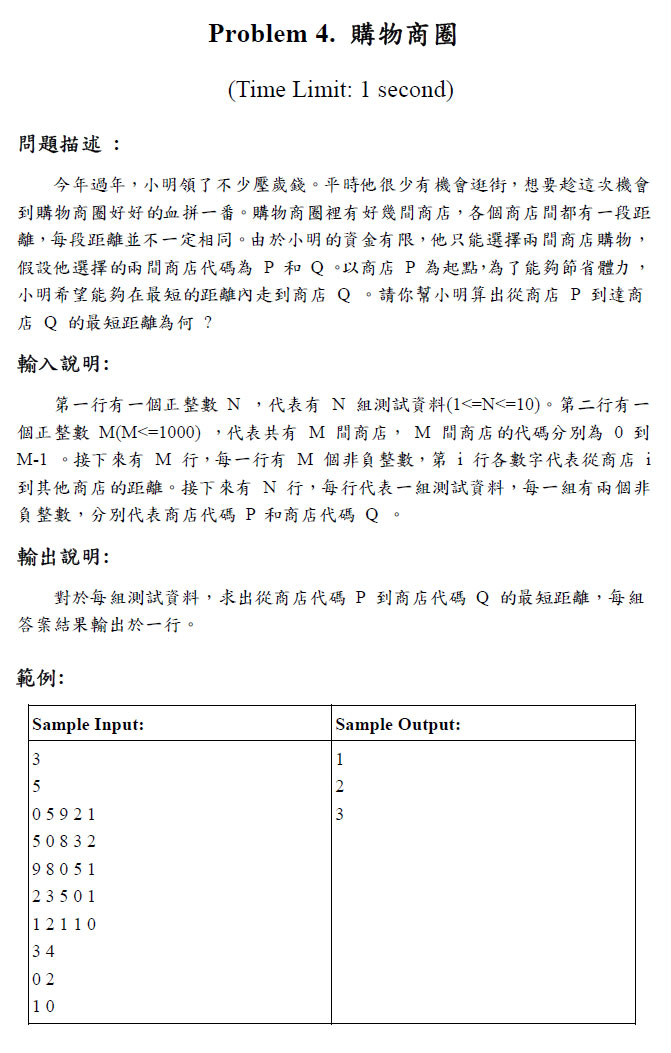
\includegraphics[height=.95\textheight]{../solutions/fig/58ITSA4}}
\subsection{解題思惟}
\begin{enumerate}
	\item m個點之間相互的距離用二維矩陣處理比較容易,因為m不會超過1000,可以宣告一個d[1000][1000]的二維陣列,其中$d_{st}$表示商店s和商店t的距離。
	\item 商店s和商店t的最短途徑要怎麼算呢?我們可以用迭代的方法思考,首先,如果直接從s到t,那麼距離就是$d_{st}$,但如果經過商店$i$,則距離會是
	$d_{si}+d_{it}$,後者有可能會比較短。前者可以看成走一步,後者可以看成走兩步。當然也有可能會有更多步,但距離更短的情況發生。
	\item 我們考慮$s$到所有$i$的最短距離,只走一步的話,就是$d_{si}$,如果走兩步的話,就要檢查所有的$j, j\ne i$,看那一個$j$會使$d_{sj}+d_{ji}$最短。假設找到$j=k$是最好的情況,那我們還要檢查看看$d_{sk}+d_{ki}$有沒有比$d_{si}$更好,如果有的話,表示走兩步的情形,會有比走一步更好的情況發生。
	\item 迭代的方式,就是從一步開始考慮,這時$s$到$i, i\ne s$的最短途徑距離定義成$d_i = d_{si}$。
	\item 接下來我們針對所有多走一步的情況,計算看看有沒有可能找到$j, j\ne s$,使得$d_{sj}+d_{ji}$比$d_i$更小,如果有的話,表示我們找到了多走一步,但距離比較短的方式,那我們就可以更新$d_i$的值。
	\item 只要有一個$d_i$的值被更新了,表示有可能有更好的途徑,我們就重複上一步驟,繼續更新所有的$d_i$。如果已經沒有任何$d_i$可以更新,那表示已經找不到更好的途徑了,那這時候$d_t$就是從$s$到$t$的最短途徑了。
\end{enumerate}

\subsection{程式碼}
\begin{cppcode}
#include <iostream>

using namespace std;

int m, d[1000][1000];

int mindis(int s, int t);

int main()
{
	int kase;
	cin >> kase >> m;
	for (int r=0; r<m; r++) for (int c=0; c<m; c++) cin >> d[r][c];
	while (kase--) {
		int s, t;
		cin >> s >> t;
		cout << mindis(s, t) << endl;
	}
	return 0;
}

int mindis(int s, int t)
{
	int dis[1000];
	for (int i=0; i<m; i++) dis[i] = d[s][i];
	bool change;
	do {
		change = false;
		for (int i=0; i<m; i++) {
			if (i==s) continue;
			for (int j=0; j<m; j++) {
				if (j==s) continue;
				if (dis[j]+d[j][i] < dis[i]) { dis[i]=dis[j]+d[j][i]; change=true; }
			}
		}
	} while (change);
	return dis[t];
}
\end{cppcode}